% !TeX root = figures.tex

\subsection*{pulley system 1}

\begin{center}
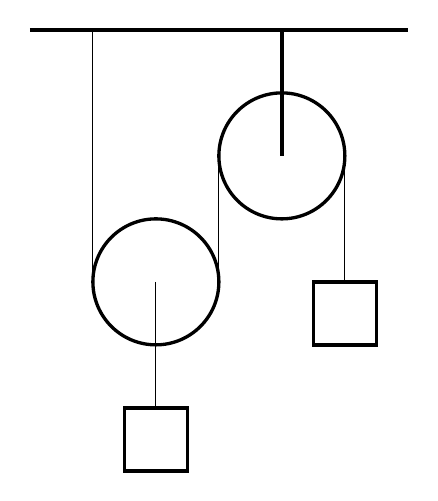
\begin{tikzpicture}[scale=0.8]

\draw [ultra thick] (0,0) -- (6,0) ;
\draw [very thick] (2,-4) circle [radius=1] ;
\draw [very thick] (4,-2) circle [radius=1] ;
\draw (1,0) -- (1,-4) (3,-4) -- (3,-2) (5,-2) -- (5,-4) ;
\draw (2,-4) -- (2,-6) ; 
\draw [very thick] (4,0) -- (4,-2) ;
\draw [very thick] (2,-6) ++(-0.5,-1) rectangle ++(1,1) ;
\draw [very thick] (5,-4) ++(-0.5,-1) rectangle ++(1,1) ;
\end{tikzpicture}
\end{center}